%23 Dec 2004
%Daniel + O
% Dominic => final

\ifx\wholebook\relax\else
\input{../Common.tex}
\input{../macroes}
\begin{document}
\fi

\chapter{Looping}\label{ch:looping}\label{cha:loops}

\begin{chapterfigure}
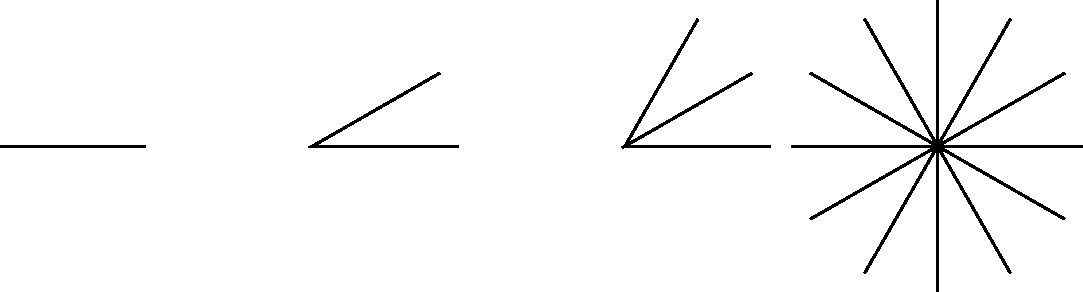
\includegraphics[width=0.9\linewidth]{loopTitlePicture}
\end{chapterfigure}

\hidden{
|\caro|
\caro := \Turtle new.
\caro west; jump: 300;east.
\caro  go: 70.
\caro  turnLeft: 180.
\caro go: 70.
\caro turnLeft: 180.

\caro jump: 150.
2 timesRepeat: [ \caro  go: 70.
				\caro  turnLeft: 180.
				\caro go: 70.
				\caro turnLeft: 180.
				\caro turnLeft: 30].
\caro east.
\caro jump: 150.
3 timesRepeat: [ \caro  go: 70.
				\caro  turnLeft: 180.
				\caro go: 70.
				\caro turnLeft: 180.
				\caro turnLeft: 30].
\caro east.
\caro jump: 150.
12 timesRepeat: [ \caro  go: 70.
				\caro  turnLeft: 180.
				\caro go: 70.
				\caro turnLeft: 180.
				\caro turnLeft: 30]
}


By now you must think that the job of robot programmer is quite
tedious. We are sure that you have ideas for nice drawings, but you don't
have the heart to write scripts to draw them.  Indeed, the amount of things to type gets larger and larger as the complexity of the drawing increases. 
  
In this chapter, you will learn how to reduce the number of expressions given to a robot by using loops. Loops allow you to \emph{repeat a sequence of messages}. With a loop, the script for drawing a hexagon or an octagon is no bigger than the one for drawing a square.

\section{A Star as a Motivating Example}
We would like a robot to draw a star as shown in the picture above. The principle is as follows: A robot has to draw a line, come back to its previous location, turn a certain angle and draw another line -- and so on. 

\scriptref{scr:line} makes a robot draw a line 70 pixels long and come back to its previous location. Note that in addition, after having drawn the line the robot points in the same direction it was pointing before drawing the line.

\begin{scriptwithtitle}{Drawing a line and coming back}\label{scr:line}
| \caro |
\caro := \Turtle new.
\textbf{\caro go: 70.
\caro turnLeft: 180.
\caro go: 70.
\caro turnLeft: 180.}
\end{scriptwithtitle}


Now to draw a star, we have to \emph{repeat} part of  \scriptref{scr:line} -- plus make the robot turn a given angle, for example 60 degrees. Turning 60 degrees means that you will get 360 / 60 = 6 branches. \scriptref{scr:star} shows how this is done to obtain a star having 6 branches without using loops.


\begin{scriptwithtitle}{A star without loop!}\label{scr:star}
| \caro |
\caro := \Turtle new.
\caro go: 70.
\caro turnLeft: 180.
\caro go: 70.
\caro turnLeft: 180.
\caro turnLeft: 60. 
\textit{\textbf{\caro go: 70.
\caro turnLeft: 180.
\caro go: 70.
\caro turnLeft: 180.
\caro turnLeft: 60.}}
\caro go: 70.
\caro turnLeft: 180.
\caro go: 70.
\caro turnLeft: 180.
\textit{\textbf{\caro turnLeft: 60. 
\caro go: 70.
\caro turnLeft: 180.
\caro go: 70.
\caro turnLeft: 180.
\caro turnLeft: 60.}}
\caro go: 70.
\caro turnLeft: 180.
\caro go: 70.
\caro turnLeft: 180.
\caro turnLeft: 60. 
\textit{\textbf{\caro go: 70.
\caro turnLeft: 180.
\caro go: 70.
\caro turnLeft: 180.
\caro turnLeft: 60.}}
\end{scriptwithtitle}

As you see, it clearly does not scale to have to repeatedly type all this code that
does  the same thing each time. Imagine if we wanted to have a
star with 60 branches like the star shown in \scriptref{scr:starsixty}! In fact we would like to be able to repeat a sequence of messages.

\paragraph{Using a  Loop.} There is a solution to this problem: use a \emph{loop!} There are several kinds of loops. For the moment the loop we present allows you to repeat any sequence of expressions a specific number of times. The method \timesRepeat  \index{timesRepeat:} repeats a sequence of  expressions a given number of times as shown in  \scriptref{scr:starloop}. \scriptref{scr:starloop} defines the same star as \scriptref{scr:star} but in a much shorter way. Noticed that the repeated expressions are surrounded by the characters \ct{[} and \ct{]}.

\begin{scriptwithtitle}{A star with a loop}\label{scr:starloop}
| \caro |
\caro := \Turtle new.
6 timesRepeat: 
     \textbf{\textbf{[} \caro go: 70.
     \caro turnLeft: 180.
     \caro go: 70.
     \caro turnLeft: 180.
     \caro turnLeft: 60 \textbf{]}}
\end{scriptwithtitle} 

\cadre{\textit{n} \textbf{timesRepeat:}
   \textbf{[} \textit{sequence of expressions} \textbf{]} repeats the sequence of expressions n times.}

The method \timesRepeat allows you to repeat a sequence of expressions a specific number of times. In \st, a sequence of expressions surrounded by the \ct{[} and \ct{]} is called a \emph{block}. 

\timesRepeat is a message  sent to an integer, the number of times the sequence should be repeated. In \scriptref{scr:starloop} the message \timesRepeat \ct{[...]} is sent to the number \ct{6}. Note that there is nothing new here as we already mentioned that even adding two numbers is done by sending message to the first one in \st. 

Finally note that the number receiving the message \timesRepeat has to be  a \emph{whole number}  because as in real life it makes no sense to do a sequence of 
expressions 0.2785 times.

The argument of \timesRepeat is a block, \ie a sequence of expressions surrounded by \ct{[} and \ct{]}. A message argument is the required information needed to make the message execution work (see Chapter~\ref{cha:firstscript}). For example \ct{[\ \caro go: 70.
     \caro turnLeft: 180.
     \caro go: 70.\ ]} is a block, that is a sequence of three expressions: \ct{\caro go: 70}, 
     \ct{\caro turnLeft: 180} and  \ct{\caro go: 70}.

\cadre{The argument of \timesRepeat is a block, \ie a sequence of expressions surrounded by \ct{[} and \ct{]}.} 


\paragraph{Loops at Work.} If you compare \scriptref{scr:line} with the expressions in the loop of \scriptref{scr:starloop}, you will see that there is one extra expression: \ct{\caro turnLeft: 60}. Can you explain why you need such an expression to draw a star? Can you draw a simple relationship between the branch number and the angle that we should turn in addition to draw a branch? 

To have a complete star the relation between the angle and the number of repetitions should be $angle * n = 360$. In  \scriptref{scr:starloop} the loop is repeated 6 times and the angle is 60 degrees, so the star is complete. 

Type \scriptref{scr:starloop} and change the number of times the loop is repeated by replacing \ct{6} by the number you want and generate a complete star.  

\begin{exofig}{loopStar60}\label{scr:starsixty}
Write a script that draws a star with 60 branches.
\hidden{| \caro |
\caro := \Turtle new.
60 timesRepeat: 
      \textbf{[} \caro  go: 70.
      \caro  turnLeft: 180.
      \caro go: 70.
      \caro turnLeft: 180.
      \caro turnLeft: 6 \textbf{]}}
\end{exofig}

\paragraph{About code indentation.}
In \st, the code can be laid out in all kinds of ways and the indentation (the spacing from the left margin  to the beginning of the line) does not change the program's result. We say it does not affect the sense of a program. However, using a clear indentation really helps the reader to understand the code. 

We suggest following the convention we used in \scriptref{scr:starloop} to format \ct{timesRepeat:} expressions and as shown in Figure~\ref{fig:loopsindent}. The idea is that the repeated block of expressions surrounded by the characters \ct{[} and \ct{]} should form a visual and textual rectangle. That is why we start the block with \ct{[} on the next line after the \ct{timesRepeat:}, align all the expressions inside the block with one tab, and finish with the \ct{]} that indicates where the block ends. 

\begin{figure}[!h]
\centerline{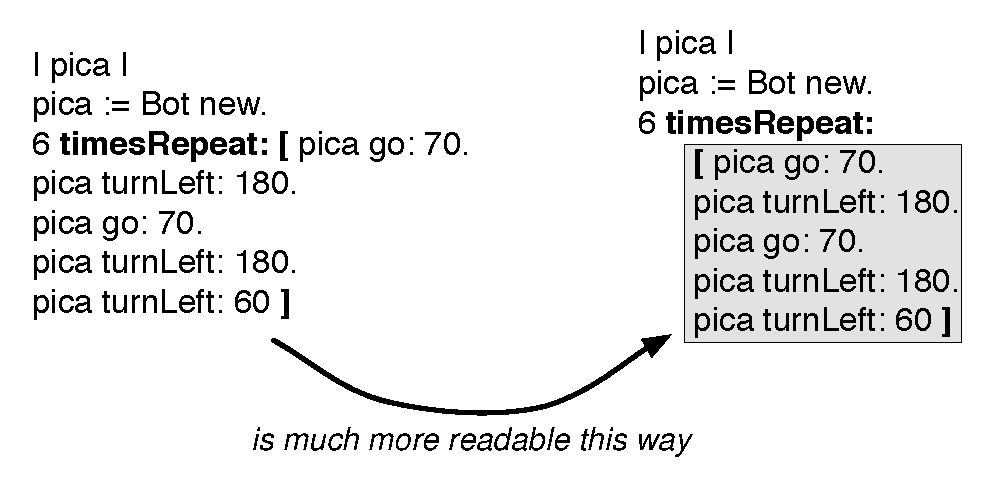
\includegraphics[width=12cm]{indent}}
\caption{The same program not indented and indented using a simple indentation to support loops identification.} \label{fig:loopsindent}
\end{figure}

Note that code formatting is one of the most complex topics because different people like to read their code in different ways. The one we propose is primarily focused at helping the reader identify the repeated expressions.



%\section{Typing in the Air}
%If you want to type \remove{directly} the code of your loops \replace{using}{directly into} the balloon, \replace{you should realize}{notice} that you need a way to \replace{tell that}{send} certain messages \remove{are sent} to the robot itself\replace{, this}{. This} is exactly the purpose of the word \ct{self} in \sq. 
%Figure~\ref{fig:fourtimesRepeat} shows how we can directly ask a \Turtle to draw a square with and without cascade. We will also see that \ct{self} is really necessary when we \remove{will} define new \replace{kind}{kinds} of messages in Chapter~\ref{ch:abstraction}.

%\begin{figure}[!h]\centerline{\includegraphics{balloonSelf4timesRepeat}}\centerline{\includegraphics{balloonSelf4timesRepeatCascade}}
%\caption{Using \ct{self} to refer to the \Turtle that will receive the messages \ct{go: 100} and \ct{turnLeft: 90}. \label{fig:fourtimesRepeat}}\end{figure}



\section{Exercising Regular Shapes}
As you may have noticed, some figures can be obtained by simply
repeating sequences of expressions, especially the ones produced in
Section~\ref{sec:firstPolygons} of Chapter~\ref{ch:relativeTurn} (repeated here as the script~\ref{scr:boucl:relativeSquare}). 

%\begin{scriptfigwithsize}[0.4]{
\includegraphics[width=4cm]{loopFirstSquare}}{A first square} \label{scr:boucl:relativeSquare}
%| \caro |
%\caro := \Turtle new.
%\caro go: 100.
%\caro turnLeft: 90.
%\caro go: 100.
%\caro turnLeft: 90.
%\caro go: 100.
%\caro turnLeft: 90.
%\caro go: 100.
%\caro turnLeft: 90
%\end{scriptfigwithsize}

\begin{scriptwithtitle}{A first square} \label{scr:boucl:relativeSquare}
| \caro |
\caro := \Turtle new.
\caro go: 100.
\caro turnLeft: 90.
\caro go: 100.
\caro turnLeft: 90.
\caro go: 100.
\caro turnLeft: 90.
\caro go: 100.
\caro turnLeft: 90
\end{scriptwithtitle}


\begin{exonofig}\label{exo:squareRepeat}
Transform  \scriptref{scr:boucl:relativeSquare} to
draw the same square but using the command \timesRepeat.
\end{exonofig}

Now you can draw other regular polygons with a large number of sides.


\begin{exofigwithsize}{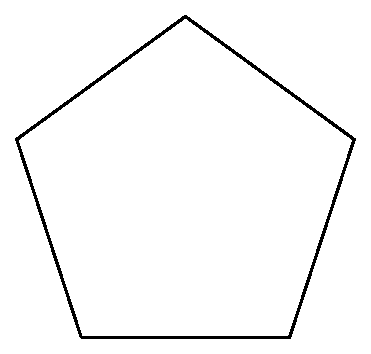
\includegraphics[width=4cm]{loopPentagon}} \label{exo:pentagonRepeat}
Draw a pentagon using the method \timesRepeat.
\end{exofigwithsize}

\begin{exofigwithsize}{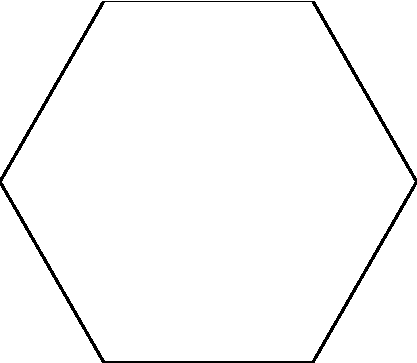
\includegraphics[width=4cm]{loopHexagon}}\label{exo:hexagonRepeat}
Draw a hexagon using the command \timesRepeat.
\end{exofigwithsize}


When you get the hang of it, try increasing the number of sides of a polygon to a very large number. You may need to reduce the length of the sides so the figure fits within the screen. When the number of sides is large and   the size of the sides is small, the
polygon will look like a circle.


\section{Pyramids Rediscovered}\label{sec:bouclonpyramids}
Remember how you coded the outline of the pyramid of Saqqarah in
\exoref{exo:saqqarah}? You can simplify your drawing by using a loop 
as follows:

\begin{scriptfig}{loopPyramid}{Pyramid script} \label{scr:pyramid}
| \caro |
\caro := \Turtle new.
5 timesRepeat: 
     [ \caro north.
     \caro go: 20.
     \caro east.
     \caro go: 20 ].
5 timesRepeat: 
     [ \caro go: 20.
     \caro south.
     \caro go: 20.
     \caro east ].
\caro west.
\caro go: 200.
\end{scriptfig}

Now you can generate pyramids with any number of
terraces \emph{with the same number of expressions}, just by changing
the numbers of the script.

\begin{exofig}{loopPyramid10} \label{exo:pyramid}
Try to draw a pyramid with 10 terraces using a variation of Script~\ref{scr:pyramid}.
\end{exofig}

You may want to generate pyramids with an even larger number of
terraces. The size of the terraces must be adjusted if you want
them to fit within the screen.

\section{Some Selected Problems}
As you have seen, the generation of the pyramid involves the
repetition of a block of code, which draws two line elements. Once the
proper repeating element is identified, one can produce complex
pictures from elementary drawings, by repetition.  The
following exercises illustrate this principle.

\begin{exofigwithsizeandtitle}{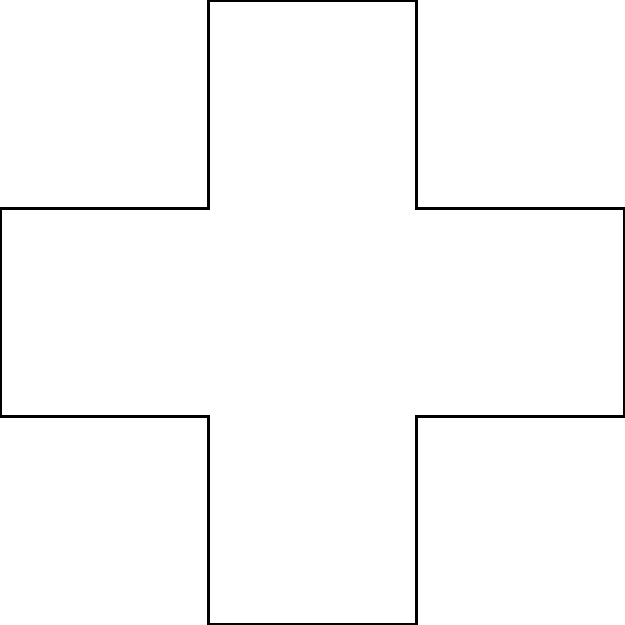
\includegraphics[width=4cm]{loopCross}}{Cross} \label{exo:redcross}
Draw the outline of the cross shown on the right using \turnLeft or \turnRight and
\timesRepeat.
\end{exofigwithsizeandtitle}


\begin{exofigwithtitle}{loopStair}{Stair}\label{exo:stair}
Draw the stairway.
\end{exofigwithtitle}


\hidden{| \caro |
\caro := \Turtle new.
10 timesRepeat: [ \caro go: 10.
                \caro north.
                \caro go: 10.
                \caro east]}

\begin{exofigwithtitle}{loopStylisedStair}{Stylized Stair}\label{exo:stylizedstair}
Draw this stylized stairway.
\end{exofigwithtitle}
\hidden{loopstylisedstair

	| \caro |
	\caro := \Turtle new.
	10 timesRepeat: [
                \caro go: 10.
                \caro north.
                \caro jump: 10.
                \caro east]}

\begin{exofigwithsizeandtitle}{
\includegraphics{loopSimpleElement}}{A Simple Element}\label{exo:element}
Draw the graphical element displayed on the right.
\end{exofigwithsizeandtitle}


\hidden{
| \caro |
\caro := \Turtle new.
\caro north. 
\caro go: 25.
\caro west.
\caro go: 25.
\caro south.
\caro go: 25}


\begin{exofigwithsizeandtitle}[0.3]{
\includegraphics{loopComb}}{Comb}\label{exo:comb}
Transform  \scriptref{exo:element} to produce a comb.
\end{exofigwithsizeandtitle}

\hidden{
| \caro |
\caro := \Turtle new.
8 timesRepeat:
 [\caro north. 
\caro go: 25.
\caro west.
\caro go: 25.
\caro south.
\caro go: 25]}


\begin{exofigwithsizeandtitle}{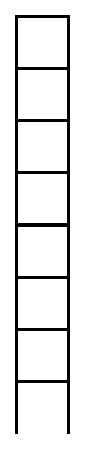
\includegraphics{loopLadder}}{Ladder}\label{exo:ladder}
Transform \scriptref{exo:element} to produce a ladder.
\end{exofigwithsizeandtitle}


\hidden{
| \caro |
\caro := \Turtle new.
8 timesRepeat: 
[\caro north. 
\caro go: 25.
\caro west.
\caro go: 25.
\caro south.
\caro go: 25.
\caro north.
\caro jump: 25.
\caro east.
\caro jump: 25]}


\begin{exonofig}
Now that you have mastered loops, define a loop that draws the tumbling squares of the picture shown at the opening of Chapter~\ref{ch:relativeTurn}.
\end{exonofig}




\summa

\begin{itemize}
\item \textit{n} \textbf{timesRepeat:}
   \textbf{[} \textit{sequence of expressions} \textbf{]} repeats the sequence of expressions n times.
\item The argument of \timesRepeat is a block, \ie a sequence of expressions surrounded by \ct{[} and \ct{]}.
\end{itemize}

\begin{table}[h]
\centering
\begin{tabular}{||p{6cm}|p{4cm}|p{4cm}||} \hline
% after \\ : \hline or \cline{col1-col2} \cline{col3-col4} ...
Method&Description&Example\\[1ex] \hline
\begin{nalltt}
n \timesRepeat
   \ct{[} a sequence of expressions \ct{]}
\end{nalltt}
     &repeats a sequence of expressions \emph{n} times
&\begin{nalltt}
10 timesRepeat: 
    [ \caro go: 10. 
    \caro jump: 10 ]\end{nalltt} \\ \hline
\end{tabular}
\end{table}



\ifx\wholebook\relax\else\end{document}\fi
